\chapter{Présentation du Framework Himalaya}
	Himalaya est un framework d'édition d'image s'inspirant des frameworks nodaux et de la technique de megatextures. Il fut conçu par l'auteur avant la
	réalisation de ce mémoire dans le but de créer un logiciel de peinture permettant l'édition non destructive, la composition non linéaire, et d'être
	compatible avec la technique de mégatexture afin de pouvoir être utilisé dans le jeu vidéo. 


	\section{Structures de données}
		Nous allons présenter ici les structures de données de base du framework. S'il est souvent difficile de justifier la conception de ces structures
		sans examiner les algorithmes qui les utilisent, il est encore plus difficile de comprendre les algorithmes sans connaitre ces structures.
		Nous avons donc fait le choix de présenter et d'expliquer tant que possible ces structures, le reste sera présenté à la section suivante qui
		vous parlera des différents algorithmes.

		Les structures et les algorithmes seront également présentés dans le langage \emph{C}, plutôt que dans des formes plus abstraites. Ceci afin de nous
		rapprocher de l'implémentation --- également réalisée en \emph{C} --- et donc de pouvoir plus facilement discuter des performances de celle-ci. 
		Il faut toutefois noter que les structures telles que présentées dans ce rapport sont plus simples que celles de l'implémentation. En effet, 
		la gestion des modèles colorimétriques est ommise, de même que des extensions propres à l'implémentation, pour permettre par exemple une
		déboguage plus facile, et l'introspection sur les données. 

		\subsection{Les Tiles}
		Comme dans bien d'autres framework, les images d'himalaya sont divisés en grilles de tiles. Un tile est donc un bitmap rectangulaire correspondant
		à une petite région de l'image. Himalaya fait un plus grand usage des tiles que d'autres frameworks puisque toute opération prend des tiles
		en entrée et en sortie. Un tile représente donc la plus petite unité de traitement, et un intérèt particulier doit être apporté à sa conception.

		\subsubsection{Structure du tile}
			Il y a trois caractéristiques importantes à prendre en compte lorsque l'on conçoit un tile:
			\begin{description}
				\item[Sa taille en mémoire]Un premier intérèt des tiles est qu'ils sont une unité de mémoire pouvant être suffisemment petite
				pour tenir intégralement dans les caches du processeur et ainsi éviter des accès cache invalides fort coûteux en temps de calcul.
				Les processeurs de différent modèles ont différentes taille de cache et différentes manières de les gérer. Plus le tile est petit,
				plus il sera rapide de les traiter sur une grande gamme de processeurs.
				
				Cependant, si le tile est trop petit, les gains réalisés par sa taille sont perdu par la surcharge de travail que doit faire le
				framework pour gérer ces tiles. 

				En outre, si tous les tiles ont la même taille en mémoire, on réduit les risques de fragmentation, et on peut faire des
				allocateurs optimisés qui allouent les tiles de manière contigue et réutilisent les tiles libérés.

				\item[Sa taille en pixel] Si tous les pixels ont la même taille en pixel, alors les images de dimensions égales seront
				toujours divisées en tiles de la même manière, ce qui rend plus simples beaucoup d'algorithmes du framework.
				la programmation des opérations en sera également facilitée. 

				Cependant, un framework moderne doit prendre en compte la gestion de modèles colorimétriques, et niveaux de quantification
				différents. La représentation d'un pixel peut donc avoir des empreintes mémoire différentes, il faudra donc choisir entre
				avoir des tiles de même taille pixel, ou des tiles de même taille mémoire.

			\begin{figure}[h]
				\centering
				\subfloat[Un tile normal]{ \label{fig:render} \includegraphics[width=0.5\textwidth]{images/tile-a} }
				\subfloat[Un tile aux canaux séparés]{ \label{fig:render-hsv} \includegraphics[width=0.5\textwidth]{images/tile-b} }
				\caption{Deux structures de tiles}
				\label{fig:tilestruct}
			\end{figure}
				\item[La répartition des pixels dans le tile] La manière commune de représenter un pixel au sein d'un bitmap est d'avoir
				toutes ses composantes placées dans des emplacement contigus. Une autre manière est de placer chaque composante dans un
				bitmap séparé. Un tile étant alors constitué de plusieurs bitmaps. L'intéret de cette technique est que les tiles de même
				quantisation ont la même taille en pixel, et les bitmaps les constituant la même taille en mémoire. Un autre intérèt est
				qu'il est maintenant beaucoup plus facile de programmer des opérations qui peuvent gérer un nombre quelconque de composantes
				par pixel. Ces deux possibilités sont représentées par le schéma~\ref{fig:tilestruct}, page~\pageref{fig:tilestruct}

				Cependant, cela implique que l'accès à un pixel nécessite autant d'accès mémoires que de composantes, ce qui ralentit 
				l'exécution du programme. 
			\end{description}

		\subsubsection{Comparaison des tiles}
			Afin de déterminer quel type de tile, et quelles dimensions sont les plus adéquates, plusieurs expériences ont été réalisées.
			Le tableau~\ref{tileperf}, page~\pageref{tileperf} représente le résultat d'expériences qui résument les concepts précedemment exposés. Dans ce tableau, deux opérations
			sont testées : \emph{colorfill} consiste à remplir une image de $8192^2$ pixels \emph{RGBA} 8bits/composante d'une couleur unie. \emph{blend} consiste 
			en fusionner deux images de $8192^2$ pixels \emph{RGBA} 8 bits/composante par opacité. Ces deux opérations 
			sont utilisées très couramment pour la réalisation de peintures. 

			Ces opérations sont appliquées selon des schémas différents: \emph{colorfill\_full} remplit tous les tiles de l'image, alors que \emph{colorfill\_single}
			remplit un tile choisit au hasard autant de fois qu'il y a de tiles dans l'image. Le même nombre de pixels est donc traité dans les deux tests,
			mais le second devra accéder régulièrement à de nouvelles zones mémoire.

			Même chose pour les operations \emph{blend} : \emph{blend\_full} fusionne les tiles des deux images, \emph{blend\_single} fusionne deux tiles
			sélectionnés au hasard, \emph{blend\_intermediate} fusionne toute l'image sur un seul tile. Ce dernier test est fort représentatif de la
			manière dont les tiles sont utilisés dans Himalaya.

			Ensuite les tiles normales sont comparées aux tiles à canaux séparés. 
			

			\begin{table*}
				\label{tileperf}
				\tiny
				\begin{tabular*}{\textwidth}{@{\extracolsep{\fill}} | r | c || c | c | c | c | c | c | c | c | c |}
					\hline
					\multicolumn{2}{|r||}{Largeur des tiles (pixel)}& 8	& 16	& 32	& 64	& 128	& 256	& 512	& 1024	& 2048	\\
					\hline 
					Test	& Canaux &\multicolumn{9}{ c|}{Temps de calcul moyen sur 5 expériences (secondes)}\\
					\hline
					\emph{colorfill\_single} & Normal 	& 0.78	& 0.64 	& 0.58	& 0.57	& 0.49	& 0.28	& 0.28	& 0.28	& 0.31	\\
					\emph{colorfill\_full} & Normal 	& 1.14	& 0.7 	& 0.65	& 0.63	& 0.55	& 0.44	& 0.47	& 0.44	& 0.51	\\
					\emph{colorfill\_single}& Séparé 	& 1.30	& 1.06 	& 1.04	& 1.06	& 0.97	& 0.79	& 0.79	& 0.79	& 0.80	\\
					\emph{colorfill\_full} & Séparé 	& 2.14	& 1.39 	& 1.16	& 1.12	& 1.10	& 1.03	& 1.00	& 1.01 & 1.01	\\
					\hline\hline
					\emph{blend\_single} & Normal 		& -	& 3.12 	& 2.98	& 3.0	& 3.08	& 4.16	& 13.58	& 19.97	& 22.60	\\
					\emph{blend\_inter} & Normal 		& -	& 5.31 	& 5.20	& 4.96	& 5.12	& 4.85	& 13.49	& 20.46	& 20.64	\\
					\emph{blend\_full} & Normal 		& -	& 5.39 	& 5.19	& 5.17	& 5.0	& 5.42	& 13.15	& 20.44	& 21.12	\\
					\emph{blend\_single}& Séparé		& -	& 6.29 	& 5.64	& 5.39	& 6.61	& 6.50	& 18.67	& 27.48	& 28.92	\\
					\emph{blend\_inter}& Séparé		& -	& 6.55 	& 5.69	& 5.50	& 6.55	& 6.74	& 20.22	& 27.77	& 27.48	\\
					\emph{blend\_full} & Séparé	 	& -	& 6.68 	& 5.82	& 5.45	& 6.59	& 6.78	& 18.39	& 27.41 & 27.23	\\
					\hline
				\end{tabular*}
			\end{table*}
			\begin{figure}[h]
				\centering
				\includegraphics[width=\textwidth]{images/tilegraph.eps} 
				\label{fig:tilegraph}
			\end{figure}
		\subsubsection{Analyse des résultats}
			On peut tirer plusieurs conclusion de ces expériences:
			\begin{itemize}
				\item Les tiles doivent être les plus grands possibles, pour diminuer le 
			nombre d'appels de fonctions, mais ne doivent pas être trop grands, sinon les problèmes de cache dégradent fortement les performances.
				Cet effet est mis en exergue par le graphe~\ref{fig:tilegraph}, page~\pageref{fig:tilegraph}, qui représente les différents
				temps de calcul du test \emph{blend} en fonction de la largeur des tiles.  
				\item Les tiles à canaux séparés sont jusque 2 fois plus lents que les tiles normaux.
				\item Le schémà d'accès aux tiles en mémoire a un impact non négligable mais plus marqué sur les tiles normaux.
				\item Le temps pour faire la fusion d'un même nombre de pixels peut différer de 970\% selon le type de tile, sa taille et la
				manière dont il est utilisé, puisque cette opération représente la grande majorité du temps de calcul du framework, ce choix
				est particulièrement important.
			\end{itemize}
			Enfin, il ne faut pas oublier que ces expériences ommettent deux facteurs importants: Le fait que la gestion des tiles dans le framework 
			est bien plus lourde, ce qui favorise les tiles plus grands, et le fait que les tiles plus petits permettent plus de précision dans 
			la localisation des opérations, ce qui permet de réduire le nombre de pixels accédés à chaque opération.

			Déterminer l'importance de ces deux facteurs requiert d'avoir des données d'utilisation du framework représentatives, par exemple
			avec des tests utilisateur. 
		\subsubsection{Structure finale}
			Le choix s'est porté sur des tiles normaux de taille fixe de $32\times32$ pixels, et ce quelque soit le modèle colorimétrique utilisé.

			À noter que pour simplifier la discussion, le reste du rapport par de l'hypothèse que tous les tiles utilisent le modèle colorimétrique
			RGBA 8bits, qui est également le seul modèle utilisé lors des tests utilisateurs. Dans les discussions suivantes les tiles
			auront donc la même taille en pixel, mais également la même taille en mémoire. 

		\subsection{Les Frames}
			La Frame est la structure de donnée qui organise les tiles. Elle doit remplir plusieurs fonctions: stocker une image gigapixel,
			stocker les mipmaps de cette image, et servir de cache aux résultats des opérations, ainsi que les mipmaps de ceux-ci.

			L'intérèt des mipmaps est que pour un coût mémoire de seulement 33\% de l'image originale, ils permettent d'accéder à une sous région
			de l'image à une échelle quelconque en un temps ne dépendant que de la taille de cette sous-région, et non de la taille de l'image. 
			Cette propriété est indispensable pour pouvoir travailler sur des images giga-pixel.
			
			La Frame est une pyramide de tile creuses. Cette structure n'est pas nouvelle et est utilisée dans la pluspart des logiciels devant
			gérer des images gigapixel et leurs mipmaps. Les formats d'échange standard des photos satellites sont par exemple basés sur ces structures.
			
			L'intérèt d'avoir une pyramide creuse est de pouvoir stocker des tiles individuels, ce qui est indispensable pour pouvoir s'en servir
			comme d'une cache.

			Il existe plusieurs structures permettant l'organisation de tiles en pyramide creuses. La plus populaire est le quadtree, et c'est celle
			qui fut choisie pour l'implémentation des Frames.

			\subsubsection{Les quadtrees}
		\begin{lstlisting}[float,caption={Définition des hlFrameNodes},frame=tb,label=lsthlFrameNode]
typedef struct hl_frame_node{
	/* abscisse du tile */
	int tx;
	/* ordonnee du tile */
	int ty;
	/* tile  */
	hlTile *tile;
	/* Noeuds enfants */
	hlFrameNode *tl;
	hlFrameNode *tr;
	hlFrameNode *bl;
	hlFrameNode *br;
}hlFrameNode;
		\end{lstlisting}
				Les quadtrees sont composés de noeuds ayant chacun une référence optionelle vers un tile, et de quatre références vers
				les noeuds enfants. 

				Chaque ensemble de noeuds de la même profondeur représente ainsi un bitmap à l'échelle deux fois plus petite que l'ensemble de
				noeuds à la profondeur suivante.

				Une définition de la structure des noeuds se trouve au listing~\ref{lsthlFrameNode}, page~\pageref{lsthlFrameNode}

			\subsubsection{Placer une image dans le Quad-Tree}
				Afin d'éviter d'avoir des Quad-Trees inutilement profond, les images sont stoquées au niveau le moins profond pouvant les contenir,
				soit $ceil( \log_2( max(size_x,size_y)/32))$, $size_x$,$size_y$ représentant la largeur et la hauteur de l'image en pixels.
				Cette profondeur est ensuite stoquée dans la Frame afin de pouvoir identifier le niveau correspondant à la résolution native.

			\subsubsection{Référencer les Tiles dans le Quad-Tree}
				Les tiles sont référencés par trois coordonnées $(t_x,t_y,t_z)$. $t_x,t_y$ représente les coordonnées spatiales du tile, $t_x$ valant
				zéro à l'extrémité gauche du bitmap, et étant positif à droite. $t_y$ vaut zéro à l'extrémité supérieure du bitmap et est positif vers le bas,
				et ce quelque soit l'échelle représentée.
				
				$t_z$ représente le niveau d'échelle. Il représente habituellement la profondeur du noeud à laquelle on trouve le tile. Nous avons
				choisi d'utiliser un système différent, $t_z$ vallant $0$ au niveau correspondant à la résolution native, et étant positif
				pour les échelles intérieures. L'intérèt de ce système est que la référence d'un tile est indépendante de sa profondeur dans
				le quadtree, qui peut changer lorsque l'on insère ou retire des tiles dans celui-ci.
				
				On peut s'intéresser à la valeur maximale de $t_z$ qui dépend de la taille de l'image stockée dans le quadTree.
				Comme nous voulons pouvoir indexer les pixels indépendemment, la largeur de l'image ne peut dépasser
				\emph{MAX\_INT}, Ce qui correspond à une valeur maximale de $t_z$ de $26$ sur les architectures 32bits, avec des tiles de 32 pixels
				de coté.
				
			\subsubsection{Les coordonnées négatives}
				Lorsque la Frame sert à stocker un bitmap chargé depuis le disque, les pixels le constituant, et donc les tiles, ont toujours des
				coordonnées $t_x,t_y$ positives. Cependant, il est pratique de pouvoir également stocker des pixels de coordonnées négatives, afin
				de disposer du plan complet pour pouvoir stocker le résultat de transformations géométriques. Pour ce faire, la Frame
				stoque un Quad-Tree par quadrant, et les tiles aux coordonnées négatives sont redirigées vers les Quad-Tree correspondant.

			\subsubsection{Le Tile de fond}
				Lorsque la frame est utilisée pour contenir un bitmap, celle-ci dispose d'un Tile de fond. Celui-ci n'est pas repris
				dans les Quad-Tree et est d'une couleur unie correspondant au 'fond' de l'image, habituellement une couleur transparente.
				Lorsque l'on tente d'accéder à une coordonnée qui ne correspond à aucun noeud des Quad-Trees, ce que l'on a atteint une zone
				correspondant au fond de l'image, et le tile de fond est renvoyé. Ceci permet de réduire l'espace mémoire consommé par les zones 
				vides des images.

			\subsubsection{Insertion, suppression et accès aux tiles}
				L'insertion, la suppression, et l'accès à un tile se fait en $O(n)$ ou $n$ est la profondeur à laquelle se trouve le tile dans 
				le Quad-Tree. Comme $n$ ne dépasse pas 26, le temps d'exécution de ces fonctions est borné, et on peut donc considérer que'elles
				ont une complexité de $O(1)$. 
				
				De plus l'insertion et la suppression augmentent ou diminuent automatiquement la taille des 
				quad-tree afin de s'assurer que la taille de l'arbre reste minimale. Ceci nécessite cependant de stocker à chaque noeud 
				sa coordonnée $t_x,t_y$, ce qui augmente leur taille de 40\%. TODO / evaluer l'espace pris.

			\subsubsection{Surchage mémoire}
				Les FrameNode ont un poids de $28$ Bytes, ce qui représente 2,66\% de la taille des tiles les plus petits(Alpha 8bit), 0.67\% de celle des plus
				communs(RGBA 8bit)  et 0.14\% de celle des plus grands(CMYKA 32bit). Dans le meilleur des cas, le stockage d'un tile ne 
				nécessite qu'un noeud, et 26 dans le pire des cas. On observe lors des tests utilisateurs qu'en moyenne le stockage d'un tile
				nécessite TODO noeuds, ce qui représente TODO pourcent.
			\subsubsection{Définition de l'hlFrame}
		\begin{lstlisting}[float,caption={Définition des hlFrames },frame=tb,label=lsthlFrame]
typedef struct hl_frame{
	/* largeur en pixel du bitmap */
	int sizex;
	/* hauteur en pixel du bitmap */
	int sizey;
	/* tile de fond */
	hlTile *bg;
	/* QuadTrees */
	hlFrameNode *tl;
	hlFrameNode *tr;
	hlFrameNode *bl;
	hlFrameNode *br;
}hlFrame;
		\end{lstlisting}
		\begin{lstlisting}[float,caption={API Publique des hlFrame},frame=tb,label=lsthlFrameAPI]
/* Place un tile dans f aux coordonnees tx,ty,tz */
void	hlFrameTileSet(hlFrame *f, hlTile *t, int tx, int ty, int tz); 
/* Enleve et renvoie le tile tx,ty,tz de f */
hlTile *hlFrameTileRem(hlFrame *f, int tx, int ty, int tz); 
/* Renvoie le tile tx,ty,tz, si il existe, NULL sinon. */
hlTile *hlFrameTileGet(const hlFrame *f, int tx, int ty, int tz);
/* Renvoie le tile tx,ty,yz si il existe, le tile BG sinon. */
hlTile *hlFrameTileRead(const hlFrame *f, int tx, int ty, int tz);
		\end{lstlisting}
				On trouve au Listing~\ref{lsthlFrame}, page~\ref{lsthlFrame} une définition de la structure des hlFrame.
				On trouvera également au Listing~\ref{lsthlFrameAPI}, page~\ref{lsthlFrameAPI}, 
				l'API publique des hlFrame.


		\subsection{L'hlImage}
		\begin{lstlisting}[float,caption={Définition des hlImages },frame=tb,label=lsthlImage]
typedef struct hl_image{
	/* Reference vers la derniere operation de la pile*/
	hlOperation *top;
	/* Reference vers la frame contenant le bitmap 
	 * a modifier */
	hlFrame *source;
}hlImage;
		\end{lstlisting}
		\begin{figure}[h]
			\centering
			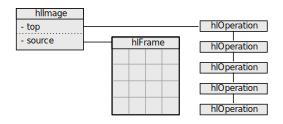
\includegraphics[width=\textwidth]{images/hlImage1} 
			\label{fig:hlImage1}
			\caption{une hlImage, avec la source et la pile d'opération}
		\end{figure}
		Si la frame représente une cache ou un bitmap, l'hlImage représente une image à proprement parler. L'hlImage est composée principalement
		de deux choses, une Frame représentant la source, c'est à dire une image de départ à modifier, et une pile d'opérations
		qui modifient l'image.	
		Une défintion de la structure se trouve au Listing~\ref{lsthlImage}, page~\pageref{lsthlImage} 

		\subsubsection{La pile d'opérations}
		\begin{lstlisting}[float,caption={API des hlImages },frame=tb,label=lsthlImageAPI]
/* Rasterise un tile de l'image */
hlTile *hlImageRenderTile(hlImage *img, int tx, int ty, int tz);
/* Insere une operation au sommet de la pile */
void hlImagePushOp(hlImage *img, hlOperation *op);
/* Enleve une operation du sommet de la pile */
hlOperation *hlImagePopOp(hlImage *img);
/* Enleve une operation de la pile et la renvoie */
hlOperation *hlImageRemOp(hlImage *img, int index);
/* Insere l'operation dans la pile */
void hlImageInsertOp(hlImage *img, hlOperation *op, int index);
/* Renvoie l'indice auquel se trouve l'operation d'uid opUid */
int hlImageOpIndex(hlImage *img, int opUid);
		\end{lstlisting}
			La pile d'opération représente l'ensemble des opérations qui vont modifier l'image source pour obtenir l'image dessinée, les opérations
			du bas de la pile s'appliqaunt en premier. Il est
			possible de manipuler cette pile par l'API publique de l'hlImage. Les opérations les plus communes sont l'ajout et le retrait d'opération
			au dessus de la pile, l'insertion et la suppression d'opérations se trouvant au  milieu. Cette API est résumée dans le 
			listing~\ref{lsthlImageAPI}, page~\pageref{lsthlImageAPI}


			Les opérations se trouvant à l'intérieur de la pile peuvent être accédées par leur indice de position dans la pile, mais aussi leur
			$uid$, identifiant propre à chaque opération. 

			La pile d'opération est implémentée par une liste simplement chainée. Chaque opération référence l'opération \emph{précédente}.
			L'\emph{hlImage} référence uniquement la \emph{dernière} opération. Les raisons de cet ordre apparaitront clairement à la vue
			de l'algorithme de rasterisation.

		\subsection{Les hlOperations}
		\begin{lstlisting}[float,caption={Définition des hlOperations },frame=tb,label=lsthlOp]
typedef struct hl_operation{
	/* Reference vers la classe de l'operation */
	hlOpClass  *class;	
	/* Reference vers l'operation precedente. */
	struct hl_operation *down;
	/* Frame qui sert de cache aux resultats de 
	 * l'operation */
	hlFrame *cache;			
	/* Reference vers l'image a laquelle appartient 
	 * l'operation */
	hlImage *image;			
	/* HL_MODIFABLE, HL_CACHING */
	int	 flags;			
	/* Un compteur de references */
	int	 refcount;		
	/* Un identifiant unique a l'operation*/
	int 	uid;
	/* Les parametres de l'operation */
	void	*params;		
}hlOperation;
		\end{lstlisting}

		Les hlOperations sont les objets qui représentent toutes les opérations qui permettent de modifier une image. Une définition de la structure
		se trouve au Listing~\ref{lsthlOp}, page~\pageref{lsthlOp}. Certaines opérations particulières pouvant étendre cette structure avec des
		champs supplémentaires, qui seront détaillés dans les sections appropriées.

		Cela représente un minimum de 32Bytes\footnote{La structure telle qu'implémentée possède de nombreux champs supplémentaires à de fins de déboguage et fait
		92Bytes} par opération sur une architecture 32bits. Une hlOperation est donc suffisemment légère pour
		que l'on puisse en utiliser plusieurs millions sans problèmes de mémoire. 

		\subsubsection{La classe d'opération}
			\begin{lstlisting}[float,caption={Définition des classes d'opérations },frame=tb,label=lsthlOpClass]
typedef struct hl_op_class{
	/* HL_COLORFILTER, HL_FILTER, HL_DRAW, HL_BLEND */
	int category;
	/* Numero de l'operation*/
	int id;
	/* le nombre de parametres flottants */
	int float_param_count;
	/* le nombre de parametres entiers */
	int int_param_count;
	/* le nombre de parametres de couleur */
	int color_param_count;
	/* le nombre de parametres d'images */
	int image_param_count;
}hlOpClass;
			\end{lstlisting}
			La classe d'opération contient la description d'un type d'opération, et tout ce qui est commun à ces opérations, Il n'existe qu'une
			seule instance de chaque classe d'opération. La définition de ces classe est donnée au listint~\ref{lsthlOpClass}, page~\pageref{lsthlOpClass}.

			Les champs des classes d'opérations méritent d'être expliqués plus en détails	
			\begin{description}
				\item[\texttt{category}]. Les opérations sont divisées en plusieurs catégories, selon les propriétés et les paramètres
				nécessaires à l'application de l'opération. Ceci permettra d'appeler une méthode spécialisée pour chaque catégorie d'opération.
				Ces catégories correspondent également aux différentes catégories d'opération de dessin que nous avons vu au premier chapitre. 
				\begin{description}
					\item[\texttt{HL\_COLORFILTER}]: Les filtres colorimétriques. Ces filtres ne sont pas dépendants de la position du tile ou de son échelle, et s'appliquent
					sur toute l'image. 
					\item[\texttt{HL\_FILTER}]: Les filtres spatiaux. Ces filtres dépendent de l'échelle, de la position du tile, 
					et ne peuvent modifier un tile sans connaitre les données des tiles adjascents.
					\item[\texttt{HL\_DRAW}]: Le dessin de primitives. Ces opérations dépendent de l'échelle et de la position du tile, 
					mais ne s'appliquent que sur une sous-région de l'image.
					 Ces filtres dépendent de l'échelle et de la position du tile, et ne s'appliquent que sur
					une sous région de l'image.
					\item[\texttt{HL\_BLEND}]] Les opéartions de fusion. Ces opérations dépendent de la position du tile et de son échelle, 
					ainsi que d'une autre \emph{hlImage}
					\item[\texttt{HL\_COLORMODEL}]] Les opérations pour lesquelles les tiles en entrée n'ont pas le même modèle colorimétrique
					qu'en sortie. 
				\end{description}
				\item[\texttt{id}]Le numéro de l'opération, qui l'identifie dans sa catégorie. Par exemple, Le dessin de cercle 
				--- \texttt{HL\_DRAW\_CIRCLE} --- dans 
				la catégorie \texttt{HL\_DRAW}
				\item[\texttt{*\_param\_count}]: Le nombre de paramètres de chaque type. Les opérations sont limitées à quatre types de paramètres,
				les flottants, les entiers, les couleurs, et les images. Cette information est nécessaire pour pouvoir calculer la taille des 
				paramètres de la fonction. L'implémentation utilise un mécanisme similaire mais plus complexe permettant une introspection sur les
				paramètres.
			\end{description}
	\section{Algorithmes}
		\subsection{Dessin}
		Dans Himalaya, le dessin et la rasterisation sont deux opérations séparées et indépendantes. Le dessin consiste simplement à ajouter une 
		opération au dessus de la pile.

		\subsection{Rasterisation}
		L'algorithme de rasterisation d'himalaya s'inspire de l'algorithme de rasterisation des frameworks nodaux, et du raytracing.
		Là ou les algorithmes de rasterisation des frameworks bitmaps et vectoriels appellent les opérations dans l'ordre avec lequel
		elles ont été ajoutées, himalaya les appelles dans l'ordre inverse; depuis la dernière jusqu'à la première.  En outre, comme dans
		le raytracing, l'algorithme de rasterisation d'himalaya peut se faire indépendemment pour chaque pixel, et donc pour chaque tile. 

		Ceci a plusieurs intérèts :
		\begin{itemize}
			\item Si une opération a son résultat en cache, on peut réutiliser ce résultat sans examiner les opérations antérieures.
			\item Si une opération est opaque, c'est à dire qu'elle masque le résultat des opérations précédentes, on peut l'appliquer
			sans examiner les opérations entérieures.
			\item Si la rasterisation d'un tile est indépendant de celui de son voisin on peut utiliser un thread par calcul de tile, et donc
			exploiter facilement le multi-thread.
			\item Si la rasterisation d'un tile est indépendant de celui de son voisin, on peut identifier les tiles de la région à visualier,
			et ne rasteriser que ceux-ci. Le temps de rendu est donc proportionnel à la région à visualiser, et non à la taille de l'image sur
			laquelle on travaille. Cette propriété est indispensable pour travailler sur des images gigapixel.
		\end{itemize}

		\begin{lstlisting}[float,caption={Rasterisation d'opérations},frame=tb,label=lsthlOpRenderTile]
hlTile *hlOpRenderTile(hlOperation *op, int tx, int ty, int tz){
	hlTile *tile = hlFrameTileGet(op->cache,tx,ty,yz);
	if(tile){
		if(hlOpCaching(op,tx,ty,yz)){
			return hlTileCopy(tile);
		}else{
			return hlFrameTileRem(op->cache,tx,ty,yz);
		}
	}else{
		if(hlOpOpaque(op,tx,ty,yz)){
			tile = hlTileNew();
			hlOpRasterise(tile,op,tx,ty,yz);
		}else{
			if(op->down){
				tile = hlOpRenderTile(
				  op->down,tx,ty,yz);
			}else{
				tile = hlTileCopy(hlFrameTileGet(
				  op->image->source,tx,ty,tz));
			}
			hlOpRasterise(tile,op,tx,ty,yz);
		}
		if(hlOpCaching(op,tx,ty,tz)){
			hlFrameTileSet(	op->cache,
				hlTileCopy(tile),tx,ty,yz);
		}
		return tile;
	}
}
hlTile *hlImageRenderTile(hlImage *img, int tx, int ty, int tz){
	if(img->top){
		return hlOpRenderTile(img->top,tx,ty,tz);
	}
	return NULL;
}
	\end{lstlisting}
		Le listing~\ref{lsthlOpRenderTile}, page~\pageref{lsthlOpRenderTile} Montre une version simplifiée de l'algorithme
		de rasterisation. Examinons le en détail :
		\paragraph{Spécification:}
		\begin{description}
			\item[pre] --
			\item[tx, ty, yz] sont les coordonnées du tile à rasteriser. Ces coordonnées correspondent aux tiles du résultat,
			et non à celles de la Frame source.
			\item[op] est l'opération que l'on désire rasteriser.
			\item[returns] l'algorithme renvoie un nouveau tile qui est le résultat de toutes les opérations de l'image antérieures
			et égales à op, appliquées sur les données de la Frame source. Il faut libérer ce tile après utilisation.
			\item[post] Le résultat de cette opération est mis dans la cache de celle-ci.
		\end{description}
		
		\paragraph{Analyse ligne par ligne}
		\begin{description}
			\item[2.] La première chose à faire est de récupérer le résultat de l'opération dans la cache. 
			\item[3-8.] Si le résultat était dans la cache, on le renvoie
			\item[4-5.] Si l'opération doit encore garder ce tile en cache, on renvoie une copie.
			\item[6-7.] Sinon on l'enlève de la cache et on le renvoie.
			\item[9-27.] Le résultat n'étant pas dans la cache, il faut le calculer.
			\item[10-12.] On fait appel à l'opération pour savoir si son effet est opaque, et donc indépendant du résultat des opérations
			 précédentes. Si c'est le cas, on crée un tile vide (ligne 7) et on applique l'opération sur ce tile.
			\item[13-22.] L'opération n'est pas opaque, il faut donc l'appliquer sur le résultat des opérations précédentes.
			\item[14-16.] S'il y a une opération précédente on récupère son résultat par un appel récursif de cette fonction sur l'opération
			précédente.
			\item[17-19.] S'il n'y a pas d'opération précédente c'est que l'on est à la première opération, qui s'applique sur la Frame Source.
			\item[21.] \emph{tile} vaut désormais le résultat des opérations précédentes. On peut donc lui appliquer l'opération en cours.
			\item[23-25.] S'il est intéressant de mettre en cache à cette opération, on met une copie du tile en cache.
		\end{description}

		\lstinline$hlOpRenderTile(..)$ n'est cependant pas accessible à l'utilisateur, puisque celui ci n'a pas d'accès direct aux opérations de la pile.
		Pour rasteriser l'image il utilise \lstinline$hlImageRenderTile(..)$ 
		
		\subsubsection{Complexité spatiale et temporelle}
		La complexité temporelle de l'application d'une opération sur un tile est de $O(1)$ puisque les tiles possèdent un nombre fixe de pixel. 
		La complexité temporelle de l'insertion et du retrait dans la chache est également de $O(1)$. Chaque appel récursif à \lstinline$hlOpRenderTile(...)$
		Se fait donc en $O(1)$. La complexité temporelle de la rasterisation d'un tile est donc de $O(n)$ ou $n$ est le nombre 
		d'opérations ajoutées au sommet de la pile depuis la dernière rasterisation de ce tile. 

		Pour rasteriser une région, de l'image, il faut identifier les tiles correspondant à cette région, et les rasteriser un par un. La complexité
		temporelle pour rasteriser une région de l'image est donc de $O(m*n)$ ou $m$ est le nombre de tiles dans la région, et $n$ le nombre d'opérations
		ajoutées au sommet de la pile depuis le dernier rendu de cette région. 

		Cette complexité est particulièrement adaptée à la peinture, puisque très peu d'opération sont ajoutées sur la pile entre chaque rendu.
		Elle est également particulièrement adaptée à l'édition d'images gigapixel, puisque la taille de l'image n'intervient pas. 
		
		L'algorithme de rasterisation ne met en cache que lorsque l'opération le requiert, et enlève automatiquement les tiles des caches lorsque
		les opérations ne le requièrent plus. Cela garantit qu'aucun tile inutile ne reste en mémoire. La complexité spatiale dépend donc du
		nombre d'opérations qui requièrent de mettre en cache. Ceci sera détaille à la section \emph{Gestion de la cache}
		
		\subsubsection{Catégories d'opérations}
		L'algorithme tel que présenté n'est pas adapté à toutes les catégories d'opérations. Les filtres spatiaux nécessitent par exemple plusieurs tiles
		résultant de l'opération précédente pour en calculer un seul. Quand aux opérations de fusion, elles nécessitent d'obtenir le tile d'une
		autre image. Ces opérations nécessitent donc un algorithme de rasterisation légèrement différents. Le fonctionnement des opérations de fusion est détaillé
		dans une section suivante. 
		
	\section{États}
		La définition de l'hlImage telle que présentée jusqu'à maintenant n'est pas complète. En effet, comment modifier la pile d'opération sans
		corrompre les caches des opérations ? Comment défaire et refaire facilement des changements dans la pile ? 
		
		Pour permettre cela nous avons besoin d'introduire un mécanisme d'état. Un état est un \emph{uid} qui nous permet de sauvegarder et rétablir la
		pile d'opération et les paramètres de celle-ci. Ainsi il est possible de sauvegarder l'état de l'hlImage, d'ajouter, d'enlever, 
		de modifier des opérations, et de récupérer l'hlImage telle qu'elle état en chargeant l'état.

		Les états sont manipulés avec les fonctions suivantes :
		\paragraph{Fonction de manipulation d'États}
		\begin{itemize}
			\item \lstinline$hlState hlStateSave(hlImage *img)$ sauvegarde la pile d'opération dans un nouvel état. 
			\item \lstinline$hlState hlStateGet(hlImage *img, hlState s)$ renvoie l'état dans lequel se trouve l'image.
			\item \lstinline$void hlStateLoad(hlImage *img, hlState s)$ rétablit l'image à un état. 
			\item \lstinline$void hlStateRem(hlImage *img, hlState s)$ supprime un état de l'image. 
		\end{itemize}

		L'API publique de l'hlImage, combinée à l'API d'état est déjà suffisemment complète pour pouvoir réaliser  un logiciel de peinture. 
		
		\subsection{Implémentation des états}
			Les états sont des références vers des opérations de l'image. Ces références sont implémentées par une table de hachage qui
			associe à chaque état une opération. 

			Une fois qu'une opération est référencée par un état, elle ne peut plus être modifiée. Il en va de même pour toute opération
			antérieure à celle référencée, puisqu'une modification de celle-ci pourrait entrainer une modification du résultat de l'opération 
			référencée.

			Pour savoir si une opération est référencée --- directement ou indirectement --- par un état, chaque opération contient un
			compteur de référence qui compte le nombre d'états les référençant. 

		\begin{lstlisting}[float,caption={Définition des hlImages avec états },frame=tb,label=lsthlImage2]
typedef struct hl_image{
	/* Reference vers la derniere operation de la pile*/
	hlOperation *top;
	/* Reference vers la frame contenant le bitmap 
	 * a modifier */
	hlFrame *source;
	/* Hashtable associant les etats aux operations */
	HashTable *statelib;
	/* Etat en cours */
	hlState state;
}hlImage;
		\end{lstlisting}

		\begin{figure}[ht]
			\centering
			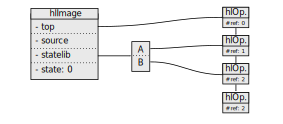
\includegraphics[width=\textwidth]{images/hlImage2} 
			\label{fig:hlImage2}
			\caption{une hlImage, avec une pile d'opérations et deux états}
		\end{figure}

			La structure de l'hlImage doit donc être modifiée pour contenir cette table de hachage, ainsi qu'une variable indiquant l'état en cours.
			Une définition de cette nouvelle structure se trouve au Listing~\ref{lsthlImage2}, page~\pageref{lsthlImage2}.
		\subsection{L'État zéro}
		Le champ \lstinline$hlImage.top$ ne change pas de fonction avec le système d'état. Cette référence pointe toujours vers 
		l'opération de l'état en cours, qui correspond à la variable 
		\lstinline$hlImage.state$. 

		Une fois un état chargé, il reste possible d'ajouter des opérations sur la pile, mais celles-ci ne sont pas sauvegardées automatiquement dans
		un état. Il est en effet totalement inutile d'avoir un état correspondant à chacune des opérations. 
		Lorsque le dessus de la pile ne correspond pas à un état sauvegardé, l'état en cours vaut la valeur spéciale \emph{zéro}.

		La figure~\ref{fig:hlImage2}, page~\pageref{fig:hlImage2} résume cette situation. On a ici deux états \emph{A,B}, et une opération non sauvegardée.
		L'état en cours vallant $0$.

		\subsection{Sauvegarder l'état}
		Pour sauvegarder un état, on crée un nouvel état, on l'associe à l'opération référencée par \lstinline$hlImage.top$ dans 
		\$lstinline$hlImage.statelib$, et on augmente ensuite de $1$ le compteur de référence de l'opération référencée, ainsi que de toutes les opérations
		antérieures. Sauvegarder l'état se fait donc en $O(n)$ où $n$ est le nombre d'opérations antérieures à l'opération à sauvegarder.
		\subsection{Charger un état}
		Pour charger un état, on commence par supprimer toutes les opérations non sauvegardées. On place ensuite dans \lstinline$hlImage.top$ une
		référence vers l'opération correspondant à l'état, et on met cet état dans \lstinline$hlImage.state$. Charger un état se fait donc en
		$O(n)$ où $n$ est le nombre d'opérations non sauvegardées.
		\subsection{Supprimer un état}
		Pour supprimer un état, on diminue de $1$ le compteur de référence de l'opération référencée, ainsi que de toutes les opérations antérieures.
		Si ce compteur vient à zéro, l'opération est supprimée. L'état est ensuite enlevé de \lstinline$hlImage.statelib$.
		Supprimer un état se fait donc en $O(n)$ ou $n$ est le nombre d'opérations sauvegardées par cet état.
		\subsection{Modifier la pile}
		Lorsqu'une pile d'opération est enregistrée par un état, on ne peut pas modifier ni les opérations de cette pile, ni l'ordre dans lequel elles
		se trouvent. Comment alors combiner le système d'état avec l'API de l'hlImage ? 

		Le principe est simple, si l'on ne peut pas modifier la pile sauvegardée, on peut en revanche modifiée une pile non sauvegardée. 
		On va donc créer une nouvelle pile identique à celle que l'on désire modifier, mais non référencée par un état.
		devient alors possible de modifier l'opération ou la pile. On appelle ce mécanisme le forking, par analogie au mécanisme
		similaire des système de contrôle de version de logiciels.
		
		\subsubsection{Le forking}
			Le forking permet de dupliquer la pile jusqu'à une certaine opération, cette opération étant antérieure ou égale aux opérations que
			l'on veut modifier dans la pile. On dit alors que l'on forke une opération.

			Voici comment se déroule le forking d'une opération.
			\begin{description}
				\item[Si l'opération à forker n'est pas référencée] Dans ce cas, les opérations suivantes ne sont pas non plus référencées,
				et rien ne nous empèche de les modifier, il n'est donc pas nécessaire de forker.
				\item[Si L'opération à forker est référencée] Dans ce cas, on va dupliquer l'opération à forker, ainsi que toutes les 
				opérations suivantes dans une nouvelle pile d'opération. Nous mettons ensuite cette nouvelle pile comme étant la pile
				courante.
				
				L'algorithme de forking va parcourir la pile d'opération 
				depuis le sommet de celle-ci. 
				\begin{itemize}
					\item Si l'opération rencontrée est non référencée, on supprime sa cache, celle-ci sera en effet
				invalidée par les modifications des opérations antérieures. 
					\item Si l'opération rencontrée est référencée, elle est dupliquée et l'opération se trouvant 
					au dessus dans la pile est modifiée pour pointer vers le duplicata. L'opération dupliquée voit 
					aussi son compteur de référence mis à zéro, et sa cache supprimée, mais garde le même uid.
					\item Si l'opération rencontrée est référencée, et correspond au sommet de la pile en cours, le
					sommet de la pile est pointé vers le duplicata de l'opération.
					\item Si l'opération rencontrée est celle que l'on désire forker, on arrète le parcourt de la pile,
					après l'avoir dupliquée.
				\end{itemize}
			\end{description}

		\begin{figure}[ht]
			\centering
			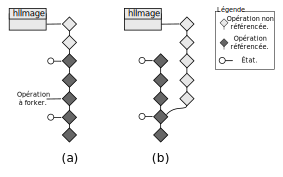
\includegraphics[width=\textwidth]{images/forking} 
			\label{fig:forking}
			\caption{Le forking d'une opération}
		\end{figure}

			Le résultat du forking est illustré à la figure~\ref{fig:forking}, page~\pageref{fig:forking}. Le schéma (a) montre la pile et l'opération
			que l'on désire forker. Le schéma (b) montre la nouvelle pile. 
			
			On constate donc que la pile n'a été dupliquée que depuis le sommet en cours, jusqu'à l'opération à forker, le reste de la pile 
			étant gardé commun, ceci permettant entre autre de réutiliser les caches des opérations communes. 

			En fait de pile, les opérations ressemblent désormais à une forèt. Mais il est impossible pour l'utilisateur du framework de s'en
			rendre compte. N'est visible depuis l'API publique qu'une simple pile et des états.

			L'intérèt de pouvoir référencer les opérations par uid apparait maintenant clair: Cela permet de référencer en tant que même 
			opération toutes les instances de celle-ci dans les différents états.  

			Le forking permet donc de concilier état et modifications pour une complexité temporelle et spatiale de $O(n)$ ou $n$ est le nombre
			d'opérations sauvegardées qui suivent l'opération à modifier.
	\section{Opération de Fusion}
		\begin{lstlisting}[float,caption={Rasterisation d'opérations},frame=tb,label=lsthlStateRenderTile]
hlTile *hlStateRenderTile(hlImage *img, hlState s, int tx, int ty, int tz){
	hlOperation *op = hlStateGetOp(img,s);
	return hlOpRenderTile(op,tx,ty,tz);
}
		\end{lstlisting}
		L'opération de fusion permet d'insérer et de fusionner un tile d'une autre image dans la pile. L'image externe doit donc être référencée par
		un état, et celui ci ne peut pas être l'état zéro, puisque celui-ci ne correspond pas à une image constante.  Insérer un tile d'une image,
		à un état spécifique implique d'être capable de rasteriser celle-ci à l'état désiré sans changer son état en cours. Ceci est fait par la
		fonction \lstinline$hlStateRenderTile(...)$ que l'on trouve au listing~\ref{lsthlStateRenderTile}, page~\pageref{lsthlStateRenderTile}.

		Cette fonction nécessite l'usage de \lstinline$hlStateGetOp(...)$ qui permet de récupérer l'opération associée à l'état, et la fonction
		\lstinline$hlOpRenderTile(...)$ que l'on trouve au listing~\ref{lsthlOpRenderTile}, page~\pageref{lsthlOpRenderTile}.
		\begin{lstlisting}[float,caption={Rasterisation d'opérations},frame=tb,label=lsthlOpBlendTile]
hlTile *hlOpBlendTile(hlOperation *op, int tx, int ty, int tz){
	hlTile *tile = hlFrameTileGet(op->cache,tx,ty,yz);
	if(tile){
		if(hlOpCaching(op,tx,ty,yz)){
			return hlTileCopy(tile);
		}else{
			return hlFrameTileRem(op->cache,tx,ty,yz);
		}
	}else{
		if(hlOpOpaque(op,tx,ty,yz)){
			tile = hlTileNew();
			hlOpRasterise(tile,op,tx,ty,yz);
		}else{
			if(op->down){
				tile = hlOpRenderTile(
				  op->down,tx,ty,yz);
			}else{
				tile = hlTileCopy(hlFrameTileGet(
				  op->image->source,tx,ty,tz));
			}
			hlImage *img  = hlBlendOpGetImg(op);
			hlState s     = hlBlendOpGetState(op);
			hlTile *tile2 = hlStateRenderTile(img,s,tx,ty,tz);
			hlBlendOpRasterise(op,tile,tile2);
			hlTileFree(tile2);
		}
		if(hlOpCaching(op,tx,ty,tz)){
			hlFrameTileSet(	op->cache,
				hlTileCopy(tile),tx,ty,yz);
		}
		return tile;
	}
}
	\end{lstlisting}
		Une fois cette fonction disponible, on peut adapter \lstinline$hlOpRenderTile(...)$ aux opérations de fusion; \lstinline$hlOpBlendTile(...)$.
		On Trouve le résultat de cette adaptation au listing~\ref{lsthlOpBlendTile}, page~\pageref{lsthlOpBlendTile}. Les modifications se concentrent
		dans les lignes 21 à 25 :
		\begin{description}
			\item{21-22.} On récupère l'image et l'état à fusionner dans l'image courante.
			\item{23.} On récupère un tile de cette image aux mêmes coordonnées que l'image courante.
			\item{24.} On fusionne les deux tiles selon les paramètres de l'opération
			\item{25.} On libère le tile de l'image externe dont on a plus besoin. 
		\end{description}

	\section{Gestion de la cache}
		La gestion de la cache peut se résmuer en deux questions :
		\subsection{Quand et où mettre un tile dans la cache}
			Plus un tile est caché proche du sommet de la pile, plus il est efficace. Le sommet de la pile semble donc
			être un endroit de choix pour cacher les opérations. 

			Il est également utile de cacher les tiles sur les opérations référencées directement par un état, puisque
			celles-ci se retrouveront au sommet de la pile dès que l'état correspondant sera chargé. 

			Si l'on sait qu'une opération sera l'objet de modifications, il peut être intéressant de cacher à l'opération
			antérieure, afin d'accélérer la rasterisation après un fork. Pour savoir quelles opérations sont fréquemment
			modifiées, on s'en remet à l'utilisateur, qui peut marquer les opérations qu'il prévoit de modifier. 

			La consommation de mémoire est donc de l'ordre du nombre d'états et d'opérations modifiables se trouvant dans la pile.
		\subsection{Quand et quel tile enlever de la cache}
			\subsubsection{Tiles invalides}
			Il y a certains tiles que l'on \emph{doit} enlever de la cache; ceux qui ne sont plus valides. Il n'existe qu'une 
			seule façon d'invalider la cache d'une opération : modifier une opération antérieure. Ces tiles sont en fait
			automatiquement supprimés par les fonctions de modification de la pile.
			
			\subsubsection{Suppression d'états}
		\begin{figure}[ht]
			\centering
			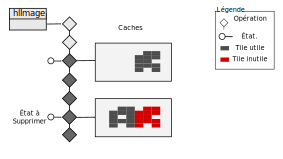
\includegraphics[width=\textwidth]{images/state-destruct} 
			\label{fig:destruct}
			\caption{Tiles inutiles après la suppression d'un état}
		\end{figure}
			Lorsqu'un état est supprimé, l'opération correspondante ne se trouvera plus jamais au dessus de la pile. On peut alors se
			demander s'il est intéressant de garder la cache de cette opération. Si l'opération ($A$) n'a pas été supprimée par la suppression
			de l'état, c'est qu'elle est référencée par un ou plusieurs autres états correspondant à des opérations ($C_i$), toutes postérieures à
			$A$. 

			A chaque tile caché de toute opération $B$, se trouvant entre $A$ et toutes les opérations $C_i$, correspond un tile caché dans $A$,
			qui est totalement inutile. En effet, tout rendu depuis les opérations $C_i$ atteindront les tiles des opérations $B$ avant d'atteindre
			les tiles de $A$. Ces tiles inutiles gaspillent de la mémoire et gagneraient à être supprimés.

			Il existe également des tiles de $A$ qui sont accessibles à partir d'une opération $C$, ceux-ci sont utiles, et gagneraient à être
			gardés. 

			Ceci est résumé par le schéma~\ref{fig:destruct}, page~\pageref{fig:destruct} qui représente en gris les tiles utiles et
			en rouge les tiles inutiles après la suppression d'un état.

			Il y a trois manières de gérer ce problème:
			\paragraph{a. Garder la cache}
				Dans ce cas, on consomme de la mémoire inutilement mais on évite de supprimer des tiles qui seront utiles par après.
				Les tiles se verront supprimés de la cache par un mécanisme global de suppression de tiles lorsque le framework manque
				de mémoire.

			\paragraph{b. Supprimer totalement la cache}
				Dans ce cas on libère toute la mémoire, mais on pourrait devoir recalculer certains tiles qui se trouvaient en cache.
				La complexité temporelle du rasterising revient donc à $O(n)$ ou $n$ est le nombre d'opération dans la pile. Heureusement,
				on atteint rarement ce cas en pratique. 

			\paragraph{c. Supprimer uniquement les tiles inutiles}
				Pour cela il faut tout d'abord trouver l'ensemble d'opération accessible depuis tous les $C_i$, ce qui n'est pas une chose 
				évidente puisque les références entre opérations vont dans l'autre sens. Dans le pire des cas la complexité spatiale
				et temporelle est de $O(n)$ ou $n$ est le nombre total d'opérations de toutes les piles correspondantes à cette image.
				La taille de l'ensemble d'opérations accessibles étant également en $O(n)$
				
				Enfin, pour chaque tile caché dans chacune de ces opérations, il faut supprimer les tiles des opérations correspondantes.
				Cette tâche se fait en $O(n*m)$ ou $n$ est la taille de l'ensemble d'opérations accessibles, et $m$ le nombre maximal de
				tile caché dans une opération. 

				Cette complexité semble prohibitive, mais il y a des cas particuliers qui se rencontrent souvent en pratique qui limitent
				fortement cette complexité. Il reste donc à savoir si les tiles utiles qui sont sauvegardés permettront 
				d'économiser plus de temps de calcul que celui qui est nécessaire pour réaliser cette opération. 

			Seules les solutions \emph{a} et \emph{b} ont été testées et implémentée. En raison de l'absence d'un dispositif global de suppression
			des tiles, c'est la solution \emph{b} qui a été retenue. 

			\subsubsection{Manque de mémoire}
			Enfin, il y a des moments ou l'on doit retirer des tiles de la cache car nous ne disposons plus de mémoire suffisante
			pour en stocker un nouveau. Aucun tile caché n'étant indispenable à la rasterisation du dessin, on peut supprimer ceux que l'on désire.
			
			Il faut donc trouver le tile le moins utile. il s'agit là d'un sujet vaste qui n'a pas encore été exploré
			ni implémenté. 
			
			Pour l'instant les tiles ne sont jamais retirés de la cache par manque de mémoire. Cela n'a pas posé de problèmes lors
			des tests utilisateurs, mais ceux-ci ne sont pas représentatifs d'une utilisation prolongée du framework. 

		\subsection{Migration de la cache}
			Il est également possible de migrer les tiles moins intéressant sur le disque dur, ou sur un espace réseau.
			Cette possibilité n'a pour l'instant pas été explorée ni implémentée.

	\section{Utilisation}
		Nous allons montrer dans cette section quelques examples qui illustrent l'utilisation de la structure et des algorithmes présentés
		dans ce chapitre afin de réaliser des fonctionalité utiles, ou d'émuler le fonctionnement d'autres frameworks. 
		\subsection{Undo / Redo}
			Pour implémenter l'undo redo, on va utiliser le système d'état. Après chaque modification de l'image correspondant à une action,
			on sauvegarde un nouvel état. On va ensuite placer cet état dans la "pile undo". 
			Lorsque la taille de cette "pile undo" dépasse le nombre maximal d'undo possible, on enlève le premier élément de celle-ci 
			et on détruit l'état correspondant. 

			Pour annuler une action, on charge l'état correspondant à une action antérieure. Pour refaire une action,
			on charge l'état correspondant à celle-ci. Lorsque l'on désire ajouter une action alors que l'on se trouve au milieu de la "pile undo",
			il faut supprimer tous les états se trouvant au dessus dans la pile. 

			Un tel système est efficace; les opérations de manipulations d'état sont suffisemment rapides pour que leur temps d'exécution
			soit imperceptible.
			
			La rasterisation après l'annulation ou le rétablissement d'une action est normalement en $O(1)$, grâce aux caches, 
			cependant, telle qu'implémentée, la gestion de la cache supprime des tiles utiles à la suppression d'états, ce qui peut occasionner
			quelques ralentissements. 
		\subsection{Modèle par calques}
		\begin{figure}[ht]
			\centering
			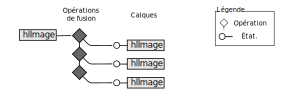
\includegraphics[width=\textwidth]{images/hl-calques} 
			\label{fig:hl-calques}
			\caption{Modèle par calques à partir d'hlImages.}
		\end{figure}
			Il est possible de construire un modèle par calque semblable à ceux utilisés par les frameworks bitmaps en utilisant les opérations
			de fusion. À chaque calque correspond une hlImage qui sera modifiée lors des peintures ou des applications de filtres. 
			Une hlImage regroupe ensuite les calques en utilisant des opérations de fusion. Ceci est représenté 
			sur le schéma~\ref{fig:hl-calques}, page~\pageref{fig:hl-calques}. 

		\subsection{Composition non linéaire}
		\begin{figure}[ht]
			\centering
			\includegraphics[width=\textwidth]{images/compnonlin} 
			\label{fig:compnonlin}
			\caption{Possibilités de composition non linéaire}
		\end{figure}
			La composition linéaire est possible grâce aux propriétés des opérations de fusion:
			\begin{itemize}
				\item Il est possible à plusieurs opérations de fusion de référencer la méme image, a des états quelconques.
				\item Il est possible à une opération de fusion de référencer sa propre image, tant que l'état référencé est antérieur
				à l'opération de fusion.
			\end{itemize}
			Il est ainsi très facile d'implémenter les \emph{history brush} qui peignent un état antérieur sur l'image ou les \emph{clone brush}
			qui peignent une copie de l'image translatée. 

			En combinant plusieurs images avec des opérations de fusion différentes, il est également possible de créer des réseaux fort complexes
			offrant des possibilités très proches de celles offertes par les frameworks nodaux. 

			Ces possibilités sont résumées au schéma~\ref{fig:compnonlin}, page~\pageref{fig:compnonlin}.

